\documentclass[letterpaper,twocolumn]{article}
\usepackage{enumerate}
\usepackage{geometry}
\usepackage{graphicx}
\usepackage[table]{xcolor}
\usepackage{tabularx}
\usepackage[backend=biber, style=numeric]{biblatex}
\usepackage{tikz}
\usetikzlibrary{external}\tikzexternalize
\usepackage{tikzit}
\input{figures/TikZiT/style.tikzstyles}
\geometry{
	letterpaper,
	left={0.75in},
	right={0.75in},
	top={0.75in},
	bottom={0.75in}
}
\addbibresource{reference.bib}
\definecolor{tableShade}{gray}{0.9}
\begin{document}
\twocolumn[
\begin{center}
	\huge\textsf{Decentralized Systems for Living Legislature}\\
	\large{Applications of Blockchain Technologies to Manage Democratized Legislation}\vspace{1cm}

\begin{tabular}{cc}\centering
	Eli Barbieri & Benn Glorfield\\
	\small{CTO, Cicero Investments} & \small{CEO, Cicero Investments}\\
	\small{elicbarbieri@gmail.com} & \small{bennglorfield@gmail.com}
	\label{title:authorSection}
\end{tabular}
\end{center}

\vspace{1cm}
]

\section*{Abstract}
	Democratized Legislation systems have governed millions of humans for decades, and much more efficiently then previous solutions like tribalism and monarchies.  There exist major inefficiencies in legacy systems, and modifying the legislation management and proposal system to utilize a blockchain could dramatically increase transparency and efficiency, while also providing a toolkit to solve future problems that may arise.
\section*{Introduction}
	Governmental systems will be around for decades, regardless of the visions of blockchain developers and enthusiasts who aim to replace everything with decentralized systems.  Judicial and Executive systems that enforce laws have major shortcomings as well, but are inherently human processes, with concrete rules being applied to unpredictable circumstances, and solving this suite of challenges is not currently possible with computational systems.  However, the management, passage, and amendment of legislation is a process perfectly suited for such systems, and the underlying technology could be utilized to give users much better control over the systems that govern them, and dramatically increase both trust and voter efficacy.
	
	A decentralized system could also transform the incentive structure, creating an ecosystem where legislators are financially and socially incentivised to act in the best interests of their constituents, and not in the interests of large capital holders.  This system, coupled with easy access and seamless user interfaces could allow for new generations of government that are more representative, trusted, efficient.

\subsection*{Content \& Deliverables}
This paper aims to lay the foundation for the development of a decentralized protocol for legislation management, transforming and optimizing the journey a bill takes from conceptualization to implementation.  Future papers will build upon these foundations, and future technical yellowpapers will define the network spec to implement the concepts addressed herein.  The following points are key takeaways from this paper, and will hopefully inspire further thought into the subject.
\begin{itemize}
\item Examine a potential network architecture that would allow for centralized management, while gaining from the benefits of decentralization.
\item Propose System that increases individual efficacy surrounding centralized legislature.
\item Describe a Framework for expansion, and an interface for solutions to future problems.
\end{itemize}

\section*{Existing Legislative Process}

\begin{figure*}\centering
	%Add California Legislative Process Fig
	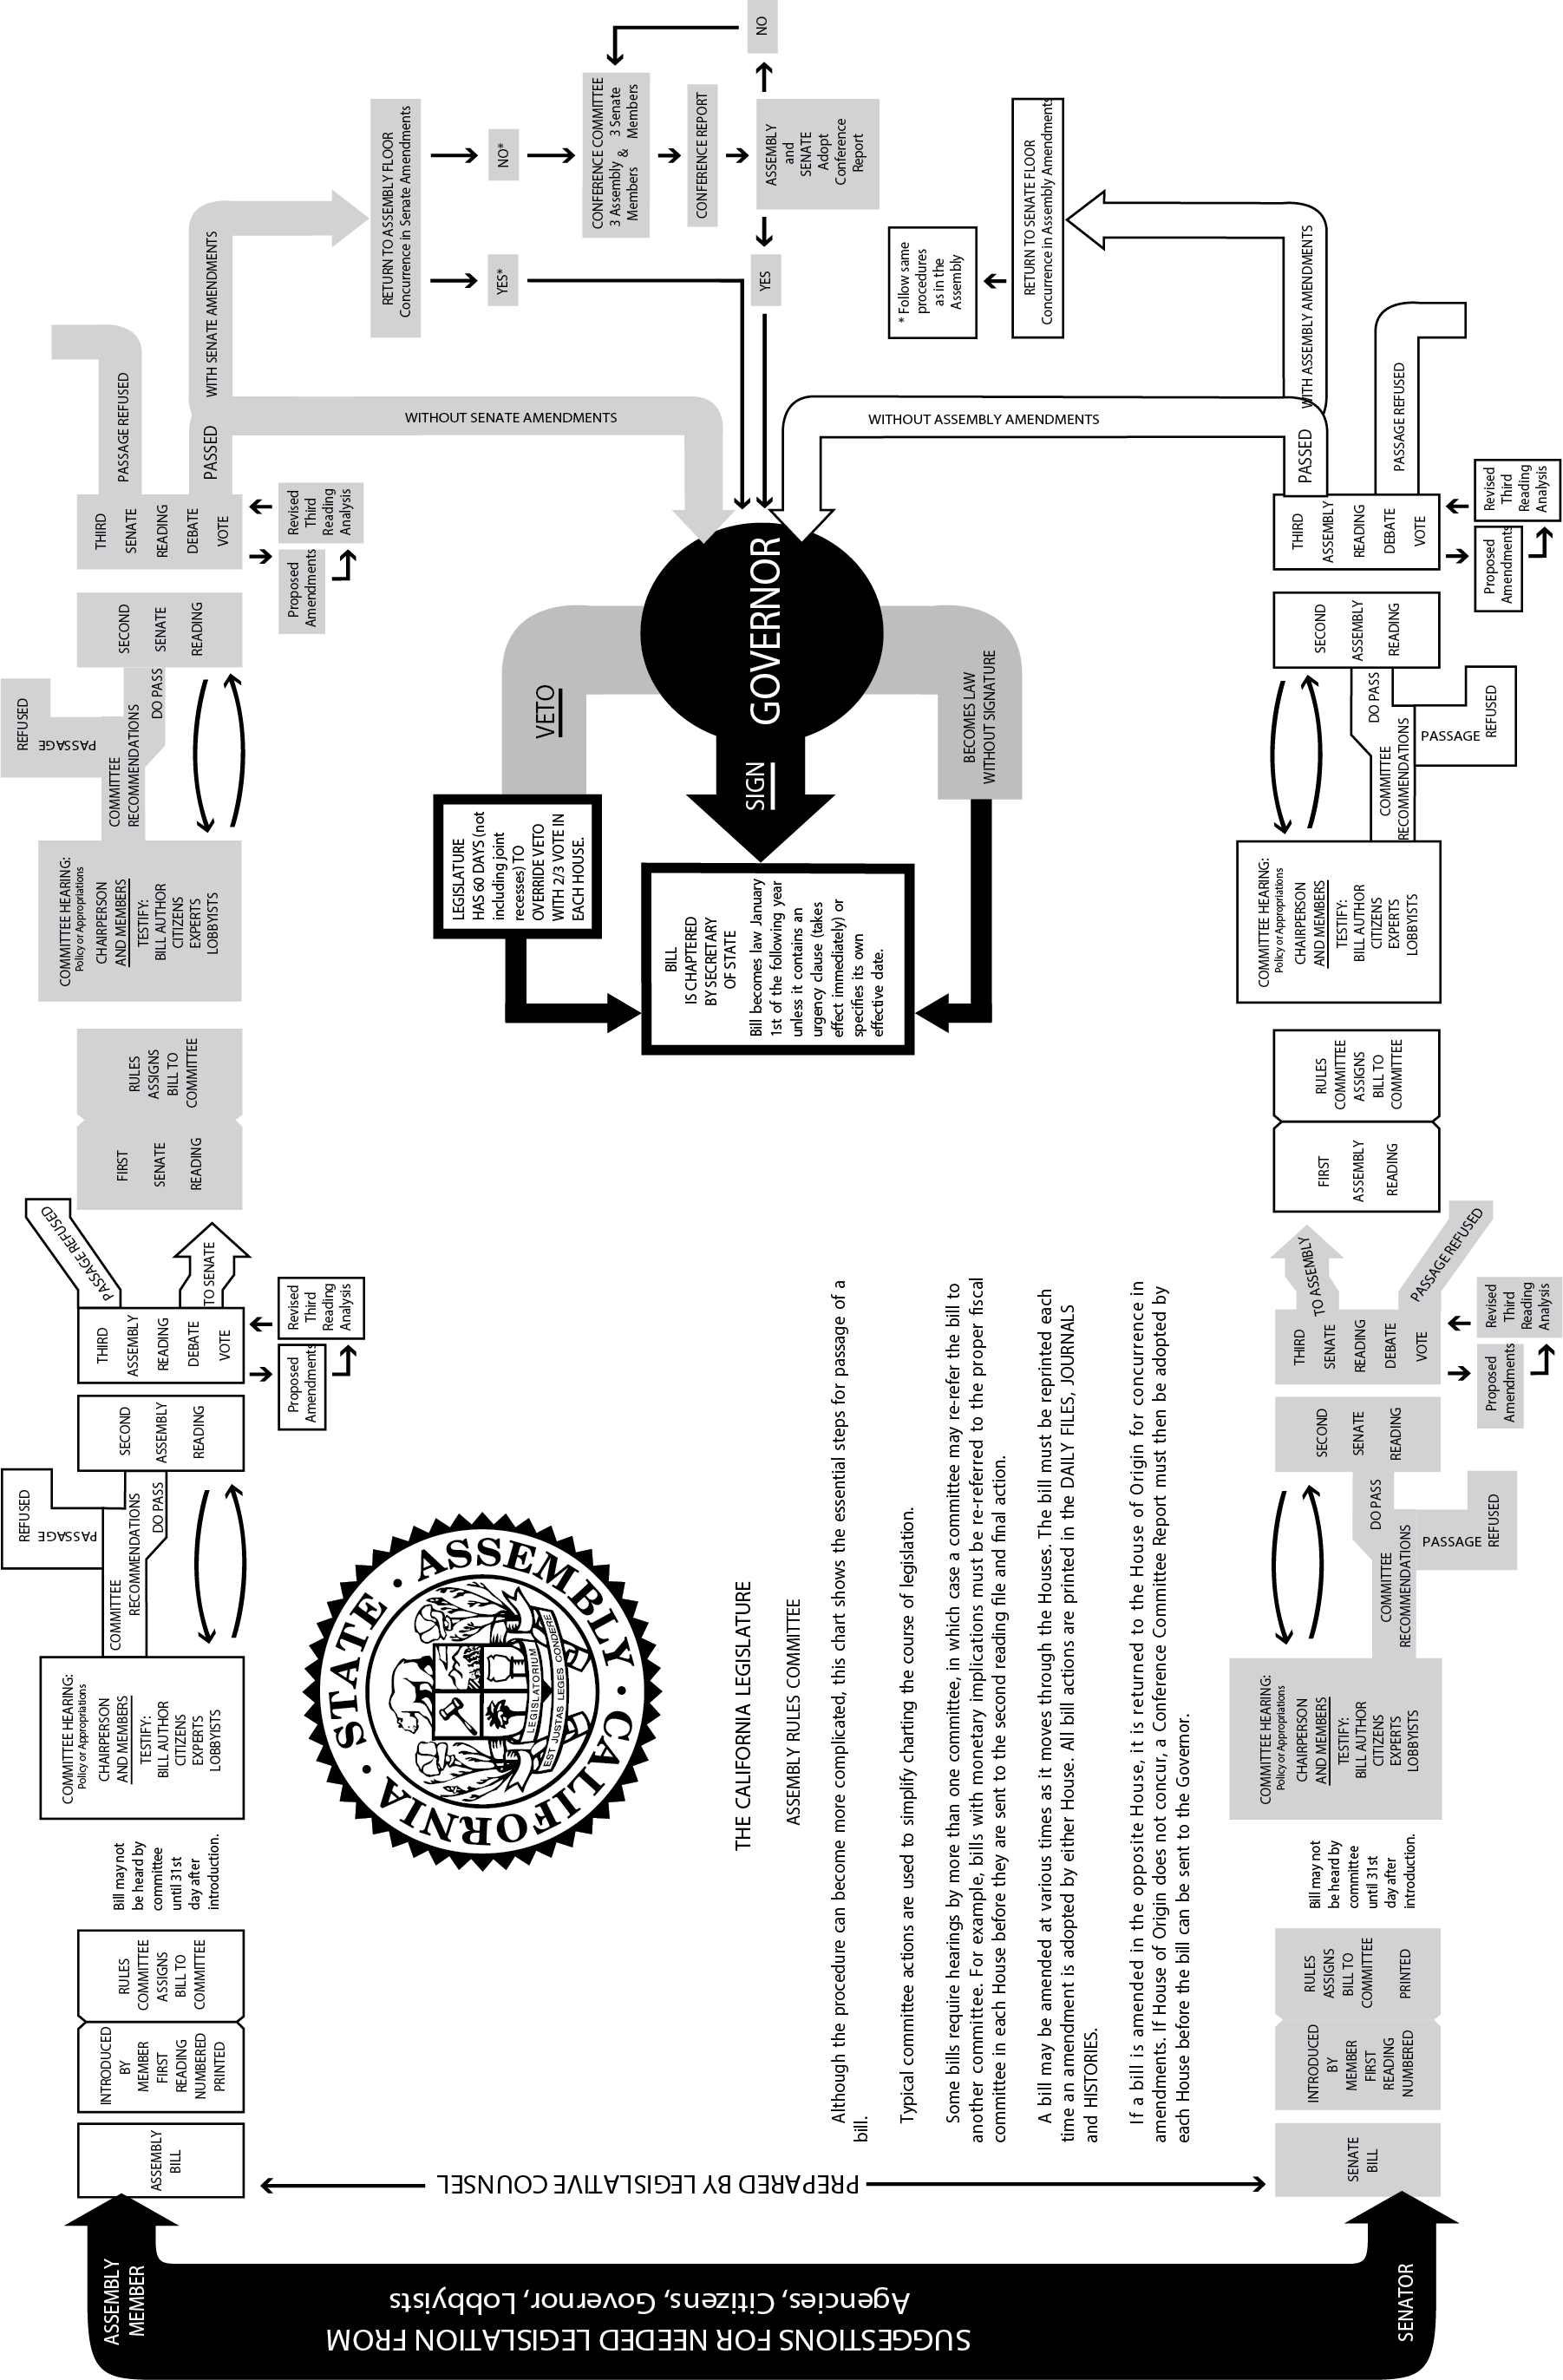
\includegraphics{figures/ca_leg.png}
	\label{fig:CA_Leg} \caption{California Legislative Process}
\end{figure*}

This paper draws upon the governmental systems of the United States, namely the California State Assembly, and the United States Federal Legislative Branch.  These processes have been modified and optimized over hundreds of years, and reflect an efficient\footnote{Efficient for a very old system that was designed without modern technology in mind} system for enacting critical legislation that impacts millions of people.  This paper examines legislative submission and enactment in the state of California, and The United States Federal Government. 

\subsection*{Legislation Proposal}
Potential bills are submitted to a legislative chamber by a sitting member, who personally sponsors the bill.  When an idea is conceived, it will be developed by the offices of legislature members were an initial draft is written, predicting the outcome and impacts.  This is formalized into a bill to be presented in front of the full chamber. Typically, the offices of legislators will work alongside private interest groups and lobbyists to develop the initial proposal. 

During the next legislative session, the proposed bill is presented to the legislative chamber where brief vote is taken to see if the proposal should be explored further.  Should a majority agree, the bill is assigned to an appropriate committee for further analysis and development.  To track the numerous proposals, each bill is placed into the "Legislative Counsel computer storage and identified by a ‘request number’" \cite{Legislative_Process}  This \textit{Request Number} is used throughout the process to track the committee assignments, reports, and votes while the bill is developed and amended before its final passage.

\subsection*{Committee Process \& Drafting}
When a committee or sub-committee is assigned to a bill, they are selected to understand and report on the impact, implementation, and cost of the legislation. Different committees focus on different subjects like educational policy, tax-code, or healthcare and human-services, and bills are assigned to the committee best suited for its regulatory purpose.  In the California Legislature, committees handle more than "7,000 bills in addition to numerous constitutional amendments and other resolutions [annually]... There are currently over 25 standing committees in the Assembly and over 20 standing committees in the Senate. They may best be described as the basic working components of the Legislature" \cite{Legislative_Process}  Committees are responsible for taking proposed legislation, and formalizing it into something implementable, for evaluating the cost and impact of potential laws, guiding the amendment process to generate bipartisan support, and correcting errors in the drafting process.  This is by far the most complex system of our legislative system, and implementing this system in a decentralized manor would likely be the foundation subsequent infrastructure is built upon.

Committees are staffed with members of legislatures, and focus on a single realm of legislation.  Naturally, in a two party system, such as the United States, there will be members of different parties, schools of thought, and talents, all sitting on a committee. Keeping the members productive is of paramount importance.  To do this, committees have a seniority structure, with a chairman to oversee the proceedings of the committee.  In the United States federal government, this is determined using a "vote by secret ballot for their committee's chairman, irrespective of that member's seniority." \cite{Senate_Committees}
%TODO: Modify above paragraph

Committees are frequently tasked with examining high-impact legislation, and to do so, call upon a variety of topic-area experts for testimony, and use that information to deepen their understanding.  These experts provide insight into the challenges and benefits, and to gain a clearer understanding of how such a bill would be implemented, and its cost to the taxpayers.  After a committee has deliberated and heard from the experts, they formalize their findings into a committee report that is published to the general public and sent to the legislature.  Each report consists of a title page that clearly addresses the target purpose of the legislation, and 7 sections examining its impact and execution. \cite{Senate_Report}
\vspace{1cm}
\begin{enumerate}[I]
	\item \texttt{Purpose and Summary} \textbullet \small\textit{  Describe the purpose of the proposed legislation, its need, and the problems it solves}
	\item \texttt{Background and Need for the Legislation} \textbullet \textit{  Analyze the problems this legislation aims to solve}
	\item \texttt{Legislative History} \textbullet \small\textit{  Analyze previous legislation surrounding this topic, its successes, failures, shortcomings, and avenues for improvement}
	\item \texttt{Section-by-Section Analysis of the Bill, as Reported} \textbullet \small\textit{  Discuss and Analyze each section of the proposed bill, examining the purpose, and identifying any potential issues in its implementation}
	\item \texttt{Evaluation of Regulatory Impact} \textbullet \small\textit{  Evaluate the impact of this legislation on current problems and likely outcomes of enforcement}
	\item \texttt{Congressional Budget Office Cost Estimate} \textbullet \small\textit{  Estimate the cost of implementing proposed legislation}
	\item \texttt{Changes in Existing Law Made by the Bill, as Reported} \textbullet \small\textit{  Analyze existing legislation surrounding this topic, and the changes this law would affect \& potential ramifications}
	
	\label{fig:committee_report_outline}
\end{enumerate}


These reports are sent to a government printing office to be officially released on websites, and added to archives.  Additionally, hard-copies are printed and sent to the offices of the legislature, and made available for purchase. \cite{Legislative_Process}  

\subsection*{Voting \& Compromise}
Following a publication, the bill is added to a list for second-reading at the next meeting of the legislature.  If a bill leaves its committee without amendments, "it is read the second time, and then sent to be compared with the original bill and, after comparison, the bill is returned to the Assembly or Senate third reading file" \cite{Legislative_Process}  This second reading is used to express the findings of the committee, and propose any committee amendments to the legislative floor.  Should any amendments be deemed necessary by the committee, these modifications will be stated at the second reading, where they will be discussed and potentially implemented.  The bill will then be once-again added to the list of second reading for the next legislative day.  "Many times, opposition to bills can be overcome by amendments submitted in committee. Amendments proposed by the committees are seldom opposed by the house, since these amendments generally are offered to correct an error in the bill or to remove opposition" \cite{Legislative_Process}  After the second reading of the bill without amendments, the bill is added to the list of third reading, where members of the legislature have additional time for a final review to determine their vote on the subject.

Following the third reading, the present members take a final vote, where a majority is required for the bill to move forward.  During this time, "a member may rise to a point of order that there is an absence of a quorum. It is then the duty of the presiding officer to ascertain whether a quorum is present. A majority of each house shall constitute a quorum to do business, but a smaller number may adjourn from day to day, and may compel the attendance of absent members. A quorum is defined as one-half plus one of the duly elected and qualified members of the house" \cite{Legislative_Process}  In a legislative house of 100 members, a quorum would constitute 51 members, and a majority of those votes must be in favor of the bill.  These votes are recorded on the role-call, alongside a list of the present members.  This role call is submitted and filed with the bill's "Request Number"

After a bill has passed, it is sent to additional houses where the above process is repeated.  A new committee reviews the legislation, and the bill is read again.  If the bill is reported out of committee without amendments, it is read a third time, where it is voted on by the other legislative house.  Should the bill pass, it will be sent to the executor for signing.  Should the committee find errors in the bill, and make a correcting amendment, the bill will be returned to the proposing house before signing.  These final steps are usually the most straightforward, as members of the legislature understand that significant changes will stop anything from passing, so any final amendments are typically minor corrections that pass without challenge.  Should the executor refuse to sign the final bill, the legislative houses can override that decision with a 2/3 Super-Majority.

\subsection*{Minority and Majority Mechanics}

In democratic governments, there is almost always a multi-party system, and juggling different ideologies and visions is a difficult task for legislative systems, as they require a majority of participants to reach consensus before enacting change.  When a group is in the minority, their legislative agenda is not completely halted, but it necessarily becomes harder to implement change.  Every bill must to strive for neutrality, and a significant portion of energy is spent tailoring the proposal to please opposing parties.  While minority governments can and have created lasting impacts, "Minority governments are slightly less successful than their majority counterparts. The greatest difference between governing contexts concerns legislative productivity. Minority governments require more time to develop legislation acceptable to opposition parties, and consequently, productivity suffers" \cite{Minority_Article}.  This mechanic does not need to be inherent to governmental systems, and a well designed and implemented system could finally separate the ideas themselves from the people that brought them forth. Such a mechanic would increase legislative productivity by making decisions about and for the ideas instead of an ideological battle between opposing parties.  Using codified\footnote{codification refers to taking existing processes, and formalizing into logical instructions for computing systems} systems, multiple levels of biases and personal hiccups could be removed, to create a more decentralized system resilient to the whims of individual people.  The majority and minority distinctions could still be made, but party-centric opposition could be removed from the equation, which would undoubtedly be a step in the right direction.

\subsection*{Data Reporting and Public Reports}

Reporting legislative activities is a crucial step in the process, and a key aspect of democratizing the legal and legislative systems.  For decades, this reporting was done by government printing offices, which printed physical copies of proceedings, reports, and proposals for lawyers and governmental agencies to purchase and review.  Over the past 3 decades, this process has moved online, and now governments maintain websites and archives to retrieve and secure this data for the public.  A decentralized legislative system would be designed with data transparency from the ground up, and accessing and researching legislation would undoubtedly be far less frustrating than our current system of ancient websites that usually feel purpose-built to make research immensely-difficult.

\subsection*{Amendment \& Interpretation Process}

When legislature is first enacted, it has passed through a bicameral legislature and the above process, and been signed by an executor\footnote{President at federal level or Governor at state level}.  This is a lengthy process, where legislation is examined, amended, and perfected, but there will always be ambiguities and unforeseen situations, and in that case, the process of interpreting the legislation is up to the courts.  The judicial system perform the difficult task of applying the word of law to a broad number of situations, and in a majority of cases, their decisions hold.  However, in a small number of cases, an appeal can be filed, which is a challenge to the original decision.  These appeals must be for one of two reasons:
\begin{enumerate} [I]
	\item Error of Law \textbullet \textit{The incorrect law was applied to the decision}
	\item Violation of Due Process \textbullet \textit{The law was applied incorrectly, and rights were violated during the process of the trial}
\end{enumerate}  
An appeal can be submitted and if deemed valid, brought before an appellate jurisdiction\footnote{Court specifically for appeal cases}, where a court will determine if the law was applied correctly, and make any clarifications to the application of the law in question.  The decisions of these courts are followed by its satellite jurisdictions, and give judges insight on how the law is to be applied in edge cases.  Each region has an associated appeals court, with the Supreme Court presiding over the state jurisdictions.  In most courthouses, one will find hundreds of volumes filled with proceedings from appellate jurisdictions, so lawyers and judges can learn from those cases and apply those precedents to their own cases.  Having this process allows ambiguities to be clarified, and appeals courts give guidance on how to apply the law.  

A precedent case must address the same legal questions, and the higher the degree of factual similarity, the more weight a precedent carries. This frequently creates a point of contention between parties where lawyers compare the current case to the precedent case to determine their similarity, also requiring the judge to perform independent research \cite{Precedent_Process}.  This process is crucial to our current judiciary system, but can be a significant inefficiency.  If existing legislation could be seamlessly reworded and clarified after appeals, ambiguities could be removed from the law instead of maintaining a complex system of precedents.  

Utilizing a codified system could improve productivity and make courts more efficient, as cases would require less historical research and precedent examination.  Additionally, "for a case to be considered binding precedent is that it must have been decided by the same court or a superior court within the hierarchy to which the court considering the case belongs" \cite{Precedent_Process}  This can lead to situations where different appellate jurisdictions interpret the same laws in different manners, and could lead to additional reporting, study, and a difficult learning curve when practicing law in different appellate jurisdictions, even when the same laws are in effect.

\section*{Background}

\subsection*{Encryption}
Encryption is a commonly used term, but understanding its fundamentals is incredibly important to grasp the mechanisms that create security in our increasing digital world.  Encryption is the process of taking binary data (1's and 0's) and manipulating it with a key to generate a completely random binary string.  This process cant be reversed without the key, and due to the complexity of encryption keys, it is computationally impossible to undo the operation.  The global standard is 32 byte keys, which is equal to $2^{256}$ different possibilities.  That number is larger than the number of atoms in the observable universe, even with every computer on earth, it would take millions of years to decrypt that level of security. When hacks occur and encrypted data is compromised, it is typically by hacking the operating system, or manipulating an administrator.  A cryptographic wallet is as secure as its owner, and in a governmental system, wallets would be biometrically locked, creating military grade security within decentralized systems.

\subsection*{Ethereum}
Ethereum is the largest VM compatible blockchain, which is a special type of blockchain that can be modified to perform an almost infinite number of different functions.  Blockchains like bitcoin are similar to spreadsheets, tracking a massive registry of different wallets, and the number of bitcoins owned by each wallet.  Every computer stores this database, so no wallet can transfer more bitcoin than it owns, and so no bitcoins can be artificially printed.   VM Compatible blockchains like Ethereum take a more generalized approach, storing a registry of wallets with ether balances with all the above functionality, but also storing a data structure called a trie that can store any arbitrary data.  These VM Compatible blockchains also have a list of instructions like ADD() and MEMORYSTORE() that can be used to perform computation and store data.  This functionality can be used to create additionally currencies on top of Ethereum that track their own registry of wallets and wallet balances, or create fully decentralized exchanges that can swap different currencies automatically.  These computer instructions are stored and run by on-chain programs called smart contracts.  When a transaction is sent to a smart contract, a computation is performed, which can range from changing data fields like wallet balances, to functions like proposing a vote to increase the fee percentage on a decentralized protocol.

\subsection*{Blocks \& Transactions}
\begin{figure}[h!]
	\resizebox{\linewidth}{!}{
		\tikzfig{figures/TikZiT/block_chain}}
	\caption{Blockchain Structure}\label{fig:block_chain}
\end{figure}
Blockchains are composed of ordered blocks, which are filled with transactions.  These transactions can perform functions like transferring funds between wallets, performing calculus functions, or updating a list of votes.  Blockchain miners take transactions, and process them into blocks, which are verified by other miners to ensure no funds are being artificially created, and data is secured.  Once a block is created, and the miners agree that it is correct, another block with new transactions is mined, and placed on top of the previous block.  The blockchain state refers to the current snapshot of all the wallet balances, and the summary of all the stored data.  Using cryptographic mechanisms, the state is tracked so that changing even 1 byte of data will change the snapshot, making it impossible to modify the blockchain state without sending a verifiable transaction.  These transactions acts as changelogs, showing what modifications were made between blocks, which is a feature that will be discussed later.

\subsection*{Decentralized Autonomous Organizations}
%TODO: Really need to refine and state the intent being examining this in depth
Decentralized autonomous organizations, or DAOs, have drastically grown in frequency and popularity over the past year, and projects like Constitution DAO\footnote{https://www.constitutiondao.com/} have made national headlines.  The underlying architecture behind such organizations proves a fascinating point of study, as they attempt to create decentralized entities with the power to allocate large pools of capital, all without a leadership structure.  The core ideas behind these organizations could easily be adapted to benefit a decentralized legislature system.  

In a decentralized organization, governance is distributed amongst token holders, and the voting token is purchasable with financial assets against a bonding curve, which dictates the dollar value of the voting token, and incentivises long term participation and early entry to the DAO. 

\begin{figure}[h!]
	\resizebox{\linewidth}{!}{
	\tikzfig{figures/TikZiT/DAO_structure}}
	\caption{The DAO Structure} \label{fig:THE_DAO_Structure}
\end{figure}

Many DAOs are designed with several leagues to split responsibilities between multiple autonomous organizations to streamline the functions of each league\cite{DAO_Whitepaper}.  The DAO aims to act as a fully decentralized venture-capital fund, investing in startups and allocating capital to its members.  A Venture League is tasked with evaluating potential investments and promising startups, while the Treasury League manages the funds of The DAO, and ensures the assets are actively managed to generate annual interest returns.  A Developer League codifies proposals, and works on the secure software crucial to decentralized systems, while a compliance league works within regulatory guidelines to ensure the decentralized organization can operate within the centralized financial sector.  

Each of these leagues is composed of several different tiers, the top of which being the core "two pizza" team.  Next, a small team of partners and advisors assists the core team directly.  A vetted community is used for formalizing ideas, and performing necessary actions like documentation.  Finally, a broader open community participates in discussion, and acts as a point of contact and interaction with the decentralized organization\cite{DAO_Whitepaper}.  None of these members are elected or formally employed, rather people join communities, contribute, learn, and grow their responsibilities over time, creating a collaborative value-add environment.

While parts of this system like a Compliance League would not be necessary in a legislature management system, the idea of multiple self-contained organizations having control over a larger body could be applied to a system where that larger body is a decentralized ledger of in-effect legislation.  Public interest groups could be implemented on-chain as DAOs, and functions like unions could be formally codified to represent its members, and create an efficient and transparent process for funding and lobbying.  The community structure of DAOs could also be implemented at many levels, creating systems where citizens are empowered to participate in the legislative system.


\paragraph{Decentralized Voting}
Token based voting is a very common model, where community members own an asset that is used in proportional representation, making each voter an invested and financially incentivised member of the community.  However, this system has its problems, the most notable being that "Small groups of wealthy participants are better at successfully executing decisions than large groups of small-holders" \cite{Vitalik_Voting}.

These problems are actively being worked on, and some of the most promising models include limited governance, where on-chain voting controls few functions, and proof of individuality, or proof of participation \cite{Vitalik_Voting}. These systems would instead be designed for representative voting based on verified individuality, much like existing democratic systems, and then also utilize token based voting for specific monetarily aligned issues.  

A legislature management system would be built around verified voting parties, like assembly or senate members, and the final votes on passing bills would be assigned to elected representatives, but there exists a need for external applications to be built that allow citizens to vote on proposals, and show their representatives accurate and seamless polling data.  Programs could also be developed which allow representatives to give up their individual vote, and instead deploy that vote to a proxy that accepted votes from their constituents and went with the majority decision.  Whatever the case, there exists major voter efficacy issues in our current system, and giving citizens a more direct and transparent voice in their government would create massive value, and help to restore trust in governmental systems.

\subsection*{Multi-Sig Wallets}
A key concept to the functioning of decentralized applications is the use of Multiple Signature wallets, or Multi-Sig.  These wallets are used to hold large pools of assets, or control risky functions of contracts like deletion or suspension.  In order to transfer funds or initiate a destructive transaction, a Multi-Sig wallet must have several different members all agree to the transaction before anything can be initiated.  These are commonly used in DAO's to control the treasury funds, and by most private companies to increase capital security and minimize risk.  Instead of manipulating one private key to steal funds, an black-hat hacker would need to manipulate several private keys, and utilize them before the other signers detected the hack and increased security.  These wallets can also control functions, like adding or removing members from a voting registry, or amending in-effect legislation.


\section*{Blockchain Architecture}
Certain features of blockchain systems are incredibly efficient, and utilizing these strengths within a legislature management system will dramatically increase the likelihood of long-term success and growth.  As described in the background section, VM Compatible blockchains maintain a "state", which acts as a high-level snapshot of all the data therein.  This feature is very well suited to legislation implementation, as there is an inherent mechanic that allows a precise moment in time to be referenced, and a full picture of all the associated data could be computed at that snapshot.  A court decision could be added to a registry of closed cases, and contain a codified reference to the laws applied to the case, and the exact state of the law at that moment in time.  Should an appeal be made, the state can be retraced to the moment of the decision, and the exact wording of the law could be reviewed.  Instead of digging through archives and checking dates on amendments, a historical reference and versioning feature is built into the system.

The blockchain state will also remain constant unless a transaction initiates a modification.  This mechanic is a core security requirement, but also creates an easy to trace change-log.  Actions like changing legislation, or making amendments have to be submitted through a transaction system, so all changes and modifications are public knowledge and viewable by all.  Such a mechanic would make it much more difficult to append unrelated clauses to legislation to please donors, or further party agendas.  Additionally, a section-by-section snapshot of all legislation could be implemented, making it instantly clear what section of the legislation was modified.  Actions like legislative research would also be streamlined, for each modification can be traced, and finding each of the committee reports and voting role-calls would be as easy as selecting the creation transaction and examining its associated data. 




\paragraph{Blockchain State}
As illustrated in Figure \ref{fig:block_chain} by the \textit{Storage State} parameter, blockchains store a snapshot of all the contained data to secure the network and reach consensus with other nodes.  This state can be referenced at any point in time, and this snapshot references every byte of stored information.  Hashes are calculated at each step, so changing 1 byte of data at the base of the trie will change its parent hash, and these parent hashes will change until the root hash itself reflects the modification.  This feature lends itself well to a decentralized living legislature management system where minor wording of laws is continuously evolving.  Court cases can reference the moment of their decision as a blockchain state, so every in-effect law could easily be examined and studied for arbitrary moments in time.  This also makes changing a single clause of a law an obvious edit, making it more difficult for big-money interests to manipulate legislation for their benefit.


\subsection*{Transaction Model}
The blockchain state is secured by the network nodes reaching consensus on the current state of the network.  All changes to the state are initiated by transactions, and as new blocks are submitted, nodes will apply the transactions to the current state until the transactions have been processed, and the state is a new number.  A transaction can send funds from one wallet to another, which changes wallet balances, and subsequently, the network state.  Transactions can also be sent to Smart Contracts, which can be thought of as programs that are run each time they receive a transaction.  These programs can perform computation, verify conditions, and store and retrieve data. Transactions can add and remove data from smart contracts, which changes the network state as well.  This allows a network model where each change is bundled as a transaction, and each computer that validates the network can apply the effects of each transaction, and then verify the resulting network state.  These transactions act as change-lists, and enable secure and decentralized systems where each modification is easily traceable, and a network participant can back-trace a piece of legislation back to its inception, and see all the associated reports and committee reports that aided in its passing. 

The transaction model of the blockchain is uniquely suited to legislative systems, as it provides an easy to interpret change-log showing every change applied to the system.  No modifications can be made without a transaction, so all edits will be easily visible, and re-playable.  If a user wants to see the exact state of the legislation on a specific date, they merely need to replay the transactions until they reach the desired time.

\subsection*{Official Wallets and Security}
A core requirement of blockchain systems is an identity verification and security system.  This takes the form of wallets, which are accounts that can store funds and initiate transactions.  A wallet consists of two parts, a public key, which everyone can view, and a private key that uses encryption to control access to your public key.  The public key is used as a reference, and data like your wallet balance are stored using this public key.  In order to send a transaction that transfers your wallet funds, you need to use your private key to verify that this transaction was sent by you, and miners can use this verification to prove that the user has access to the funds in question.  This mechanic is used with all transactions, so actions like casting a vote in favor of legislation would require a private key to sign.  

In order to keep this key safe, it would need to be kept off of all servers to protect against a data breach.  Using a hardware wallet, which is a physical copy of the key is already a lot safer, and is similar to the level of security implemented in government agencies like the National Security Administration.  However, security can even further be increased by utilizing biometrically locked hardware wallets.  Finally, storing these wallets in a vault at the capital would be a logical step that would not decrease productivity, while significantly improving security.  These biometric keys would be accessed during legislative sessions for members to vote and perform management functions, and securely stored in a vault during weekends and holidays.


\subsection*{Legislative Consensus Process}
In a decentralized legislature management system, registries would be used to track legislative items, and act as the basic building blocks for a conception to implementation pipeline.  The first registry would track potential legislation, where proposals for new bills would be submitted.  This submission process would require either a high-level user (Member of the Legislature) or a large number of community signatures to add a new proposal to the registry.  This would enable independent 3rd parties to create and sponsor a bill, and remove partisan labels.  This would also help disenfranchised citizens, who instead of going to a legislator and being ignored, could create a proposal and petition the required signatures until the bill was automatically submitted to the registry.

\begin{figure}
	\resizebox{\linewidth}{!}{
	\tikzfig{figures/TikZiT/legislature_lists}}
	\label{fig:voting_amendmant_process}\caption{Basic Voting and Drafting Model}
\end{figure}

After a proposal has been submitted, a committee-like organization would review, and formalize into a legal text, and prepare a draft for voting, much like governmental committees in modern systems.  These formalized proposals would be transferred to the second legislature registry of \textit{Voting Legislation}, where elected members vote on proposals.   If a majority votes to pass, the legislation would be moved to the third registry containing the \textit{In-Effect} legislation.  Should the elected members instead vote to amend, the proposal would be moved back to the first registry.  A committee would then re-examine with the attached notes, where it would again be examined and formalized.  The proposal would then be moved to the \textit{Voting Legislation} registry, where it would wait until another vote, much like the existing legislative systems.

\subsection*{Permission Structure}
Creating a full-fledged legislation system will inherently require different levels of permissions for different network participants.  In most DAO's, all members are identical, and new proposals have a very long voting period, and take a long time to implement.  In governmental systems, it is necessary for certain actions to be restricted to elected officials, and legislative proposals like budgets and disaster relief need to be passed rapidly.  To achieve this, a decentralized system would maintain a ledger of high-level permissions, and list the wallets that are able to utilize those functions.  Performing sensitive actions on-chain would all be checked by first querying the permission contract, and verifying that the account submitting the transaction is verified to change the network state.  For example, if an elected member was to place a vote against a proposal, they would first access their biometrically locked wallet, and initiate a transaction with their vote against, and the target legislation.  This transaction would be sent to the voting contract, which would check if the sender wallet is an elected member, then submit the vote if all the conditions were met. 


\subsection*{Storage and Data Persistence}

Storing a comprehensive database of legislative activity would be a key benefit of such a system.  However, in blockchain systems, data storage comes at a cost, as very large blockchains are more expensive to run, and inherently more centralized.  Currently, the vast majority of government documents are stored as PDF files, due to their widespread support and customizability.  However, PDF files are large, and use many more bytes of data than other similar document formats.  One feature of the blockchain is it creates a secure storage space where data cannot be accidentally edited, and all modifications are fully traceable and revertible.  Because of these features, it would only be logical to utilize file formats better optimized for storing text, and basic formatting instructions as shown in Figure \ref{fig:file_formats}.

\begin{figure*}[h]\footnotesize
	\rowcolors{3}{tableShade}{white}  %% start alternating shades from 3rd row
	\noindent\begin{tabularx}{\textwidth}{@{\extracolsep{\fill}}X|X|X|c|c}
		\textbf{File Format} & \textbf{Benefits} & \textbf{Drawbacks} & \textbf{Storage Efficiency} & \textbf{Difficulty}\\
		.docx (Microsoft Word) & Fantastic Editors & Very Few & Medium & Easy\\
		.pdf (Portable Doc Format) & Can represent any content & Hard to edit \& modify & Poor & Easy\\
		.txt (Plain Text) & Super simple & No Formatting & Fantastic & Very Easy	\\
		.tex (Latex) & Infinite Configuration & Requires Compiler & Medium & Very Difficult \\
		.md (Markdown) & Practical Formatting & Slightly Limited & Fantastic & Easy \\
		.html (Hypertext Markup) & Perfect for Websites & Complex Formatting & Medium & Medium \\
		.epub (eBook) & Easy to Export & Complex Formatting & Medium & Medium\\
	\end{tabularx}
	\caption{Text Document File Formats}\label{fig:file_formats}\normalsize
\end{figure*}

%Lol is this true
In legal documents, the most utilized formatting tools are heading and section titles, and referencing existing cases and legislation.  File formats like MarkDown would be perfect for such systems, as it provides easy and efficient formatting, almost no learning curve, and a great deal of customization.  A valuable feature to add to a blockchain file spec would be a reference/hyperlink feature that could reference other on-chain data, and link to that reference, and the snapshot of that document at the time of publishing.  This data would be easily render-able from an online browser, removing the frustrating process of finding the legal documents referenced.  Such a system could provide the vast majority of formatting and text editing features professionals are accustomed to, all while using half the hard drive space, and dramatically increasing network efficiency.

A key benefit of a ground-up implementation would also be the ability to create clear standards for document formatting.  While there are guidelines for the structure of legal documents, a simple search will reveal half a dozen different formats used for the same type of document between several regions and jurisdictions.  While this is little more than an inconvenience, standardizing file formatting is a great practice, increases efficiency, and decreases headaches.

The Data-Storage problem in particular is perhaps the biggest obstacle in such a system, as storing large comprehensive databases is of great value to all participants, but also makes a decentralized implementation more difficult.  Ethereum in its current state could not support such a system operating on its nodes at the moment, and while there are massive scaling efforts underway, legislation management systems might be better suited to custom blockchains where the sole purpose is the management of legislature and associated functions.  Such a system could be more efficiently optimized for increasing governmental transparency, and would not be subject to external market factors like high transaction fees during periods of product launches.



%Elaborate on the use of custom blockchains at a later date
%\section*{Implementation}
% Custom Blockchain Arguments: Less Congestion, Meme coins cant stop trial, More Controllability and Network Wide Opportunities, Modifying Client Specifications
% Ethereum Contract System Arguments: Increased Security & Community Trust, Better Transparency tools

The core function of this system would be to provide the minimum viable infrastructure to replace the crucial functions of our current legislation management and submission system, and provide an interface for future expansion and iteration.  The core legislative tables would act as the management system, and everything else would be built around these using a VM Compatible blockchain that references legislative ID's, snapshots of In-Effect legislation, and registries like elected members.  The extensibility of this system could enable a new host of applications, and incentivise iteration and innovation in governmental systems.


\section*{Security Considerations}

Naturally, with any system that creates significant value, there will be an incentive for malicious actors to manipulate and exploit the system.  Traditionally in politics, this has been isolated to members of legislatures causing problems in protest, intentionally trying to overwhelm the system, or refusing to perform their duties.  This is a good model from a security standpoint, as only vetted and elected members pose any significant risk to a functioning legislature, but in a decentralized system, the responsibility of governance can be shared between many actors, and the number of people who can have an influence on the system is naturally much larger.

\subsection*{Legislative Spamming}
One possible attack would be a "spamming" of the legislative lists, where a malicious community with enough signatures, or rouge elected members attempted to overload the system by submitting thousands of proposals.  This could have the effect of bringing all progress to a standstill, and has been a significant problem in the past.  Before a change to the California constitution in 1958, all bills submitted after the constitutional recess required a 3/4 approval to make it to committee.  This created a system where "more than 6,700 bills were introduced in the Legislature during the 19 days before the recess" \cite{Legislative_Process}.  Soon after, actions were taken to avoid this, and there is now a "limit on the number of bills that can be introduced in a two-year session. A Senator may introduce a total of 50 and an Assembly Member no more than 40 bills" \cite{Legislative_Process}.  Similar policies could be implemented in a decentralized system, limiting the total number of proposals that can be made by an elected member, and requiring all bills brought forward by communities to have a lockup period where a verified member cannot endorse another proposal until a two week window has passed.  This would make it practically insane to try and submit more than a 4 or 5 bills every 2 weeks.

\subsection*{Court Packing \& Citizen Packing}
A potential vector for manipulation would be to artificially create hundreds of new "fake" citizens and use these wallets to perform actions in mass, like suggesting proposals and clogging the network.  This could be avoided by utilising a verification system, much like anti-bot measures on websites, to prove that the wallet owner is unique, and that the person only owns a single wallet with their voting access. Proof of individuality is an ongoing area of blockchain research, and regardless of its success, a governmental blockchain for living legislature could trivially implement a verification process utilizing government documents like passports and birth-certificates.

\subsection*{People Hacking and Social Engineering}
By far, the biggest risk in such a system will be hacking the people, and not the technology.  As has been demonstrated in past elections, and unequivocally proven in academia; social media networks have influence over people, and malicious use of these networks poses real dangers.  Additionally, a likely vector of attack would be compromising the private keys of wallets, and gaining access to the functions therein.  It is impractical for average citizens to maintain the level of security demanded by elected members, but owning a physical hardware wallet increases safety tenfold, and is also easier to use.  A key facet of a decentralized system would be ensuring that its constituents understood at least the basics, and knew where to get started, and how to find the resources to participate in such a system.

\subsection*{Private Key Compromisation \& Loss}
In the unlikely event that a private key is compromised or lost, the functions and data associated need to be recoverable. One possible solution would be to utilize a unanimous multi-sig of top level wallets to disable compromised addresses and create new wallets.  This process would likely never be used, but there would be a fully formed recovery pipeline ready just in case.  Should a citizen loose access to a private key (a likely event), there would be a form to fill out and submit, and after the documents have been reviewed, 2 or 3 elected officials could sign off on the key deactivation and renewal of the citizen wallet


\section*{Benefits \& Future Expansion}

Throughout the existing legislative timeline, public reports are created at several steps, and the tracing and management of these proposals is a difficult challenge, and a very expensive function, costing taxpayers tens of millions annually. To date, there have been 118 website contracts totaling over 5 million dollars issued by the US Federal government, and there have been 5 contracts each totaling over 100 million dollars \cite{US_Spending}.  This cost both represents a steep initial setup fee, as well as significant long-term maintenance costs. 

A decentralized management system would present upfront costs and challenges, but after its initial development and adoption period, the system would begin to manage itself, and create a far more efficient experience.  Government websites are frequently outdated, clunky, and difficult to navigate.  A key benefit of blockchain systems is the ease of data interfacing, and in the case that government-provided interfaces became unmaintained, third parties could easily build services on-top of the blockchain, and create their own legislative explorers and user experiences.


\paragraph{VM Compatible Blockchains}
As mentioned previously, the expansion opportunities presented by such a system are its greatest benefit.  With a complete instruction set, there are almost no limits to what can be done on-chain, and regardless of what issues arise, there will be a full toolkit to design and implement a solution. Updates and new features can seamlessly be coupled with existing infrastructure. Below are a number of potential applications that could be built on top of such a system, and a simple example of the potential classes of problems this system would aid in solving.

\subsection*{Polling \& Community Feedback}

In current systems, representatives typically only hear the voices of their constituents when they are mailed, called, or when conducting polls and surveys.  While sometimes adequate, this is not a modernized process, and better feedback mechanisms could be implemented with a VM Compatible blockchain.  This system would reference items in \textit{Proposed Legislation} and \textit{Voting Legislation}, and provide a registry to track community votes.  This list of community feedback is highly secure, so any data generated would likely be more reliable than existing methods like polling.  These feedback systems have the potential to dramatically increase voter efficacy, and build a feedback cycle that helps guide representatives.

\subsection*{Transparent Lobbying and Bribing}

It goes without saying that financial incentives in politics need to change, and wealthy participants have too much power over the system.  There have been numerous attempts to regulate and stop these practices, but there always seems to be loopholes and ambiguities.  With a decentralized system, a different approach could be taken, instead of making all lobbying illegal, aiming to make it completely transparent.  If a law was passed stating that any and all financial lobbying was to occur on-chain as direct bonuses to key legislators, and any other form of compensation, gifts, and dinners were illegal bribes; lobbyist efforts would likely move on-chain where every donation was traceable, and the originating party could not hide behind shell companies and legal documents.  

This would change the financial landscape of politics, and would move away from an opaque model where powerful parties influenced our laws behind closed doors, to a model where all financial incentives are viewable and public.  This also leads nicely to communities, since this lobbyist reward could just as easily be generated by a DAO.  In 2021, a DAO raised 43 million dollars to purchase an original copy of the constitution, and the average contribution was less than a thousand dollars, with tens of thousands of participants.  This speaks to the power of like-minded communities, and if given room to thrive, public interest groups could affect legislation as effectively as private companies.

Charities and non-profits could structure themselves as a league of DAOs, and its core members could vote on actions like purchasing land to restore, or sponsoring green-energy legislation.  These organizations could also integrate with community feedback contracts, and allocate their capital to enact the most widely supported legislation.  All funding expenditures would also be completely transparent, and a very high level of trust could be built around these humanitarian DAOs

\subsection*{Transparent Financials}

Governmental funds could also be moved on-chain, and processes like the state budget, and government employee salaries could be transparently distributed.  Instead of tracking spreadsheets of expenditures and awarded contracts, this data could be available in the form of transactions, which act as automatic change-lists.  Financial trails would also be more transparent than ever, enabling citizens to track each item on the budget, its sub-items, the different contractors and awards, and even where the contractors transferred the funds. 

\subsection*{Hybridized Voting}
One of the most promising benefits of such a system would be to create a hybrid model, where legislation could be enacted through both representative and direct votes.  Such a system would allow for a government representative to handle maintenance legislation like changing garbage collection protocols, or paying a contractor to retrofit an older building with handicap railings.  However, when major issues arise, like healthcare or changing an education standard, the vote would instead be decided by a direct vote of citizens.  This system would allow for housekeeping legislation to proceed unhindered, and on track, while also allowing citizens to voice their opinions directly on the big-ticket issues.

\section*{Conclusions}

\begin{figure*}[t]
	\resizebox*{\linewidth}{!}{
		\tikzfig{figures/TikZiT/final_network_diagram}}
	\caption{General Legislative Management Structure} \label{fig:legislative_structure}
\end{figure*}

The United States has built a robust and effective government that has lasted for hundreds of years, and reamained functional throughout tumultuous times.  However, our world is changing more rapidly than ever, and the system is strained under the pressure.  Blockchain systems are growing in popularity, and cryptocurrencies are beginning to become a mainstream asset class.  The tools and technology brought forward by blockchain will probably change the world forever, and the risk to reward ratio for implementing a decentralized system is appealing.

Utilizing a VM Compatible blockchain with 3 legislative registries, a full suite of functions can be built on top, as shown in Figure \ref{fig:legislative_structure} has the potential to transform numerous aspects of the legislative system.  The development and testing of such a system would undoubtedly be difficult, but a challenge that has the potential to generate a dramatically better system.  It will be crucial to build up test cases, and allow these ideas to be further explored.

These systems could be integrated into corporations to manage their employee handbook, sexual harassment policies, and their payment tables.  There are many aspects of human relations and management that accrue significant costs, and instead replacing many of those roles with a decentralized system could be a major benefit for some companies.

Decentralized legislature systems could also be fantastic opportunities for colleges, allowing political science students to learn about the legislative process, and learn about cutting edge systems.  Such a program would also create opportunities for computer science students to learn about blockchain principles, and architect decentralized networks.  These skills are invaluable in the production settings, and studying these systems in rigorous academic settings would further develop their viability.

Finally, legislature systems could be implemented in unstable countries, where rampant inflation and changes in leadership cause a majority of the country to be impoverished.  Creating a decentralized, stable, and secure system to manage laws alongside cryptocurrency assets as the reserve currencies could have a massive impact on millions of lives.  The ultimate goal of decentralized systems is to create a better future, and improve the quality of life around the world.  With blockchain as the base operating system for our human experience, the future looks a lot more promising.

\vspace{1 cm}
\printbibliography
\end{document} 